\section{Hg-High Linie}
Im nächsten Schritt soll die Linie der Quecksilberhochdrucklampe Lampe untersucht werden. \\
Im Folgenden sind zuerst einmal Darstellungen des Interferogramm der Hg-High Lampe und 
deren Einhüllende zu sehen. Die Messeinstellungen sind dem Protokoll, im Anhang, zu entnehmen. \\
\begin{figure}[h]
    \centering
    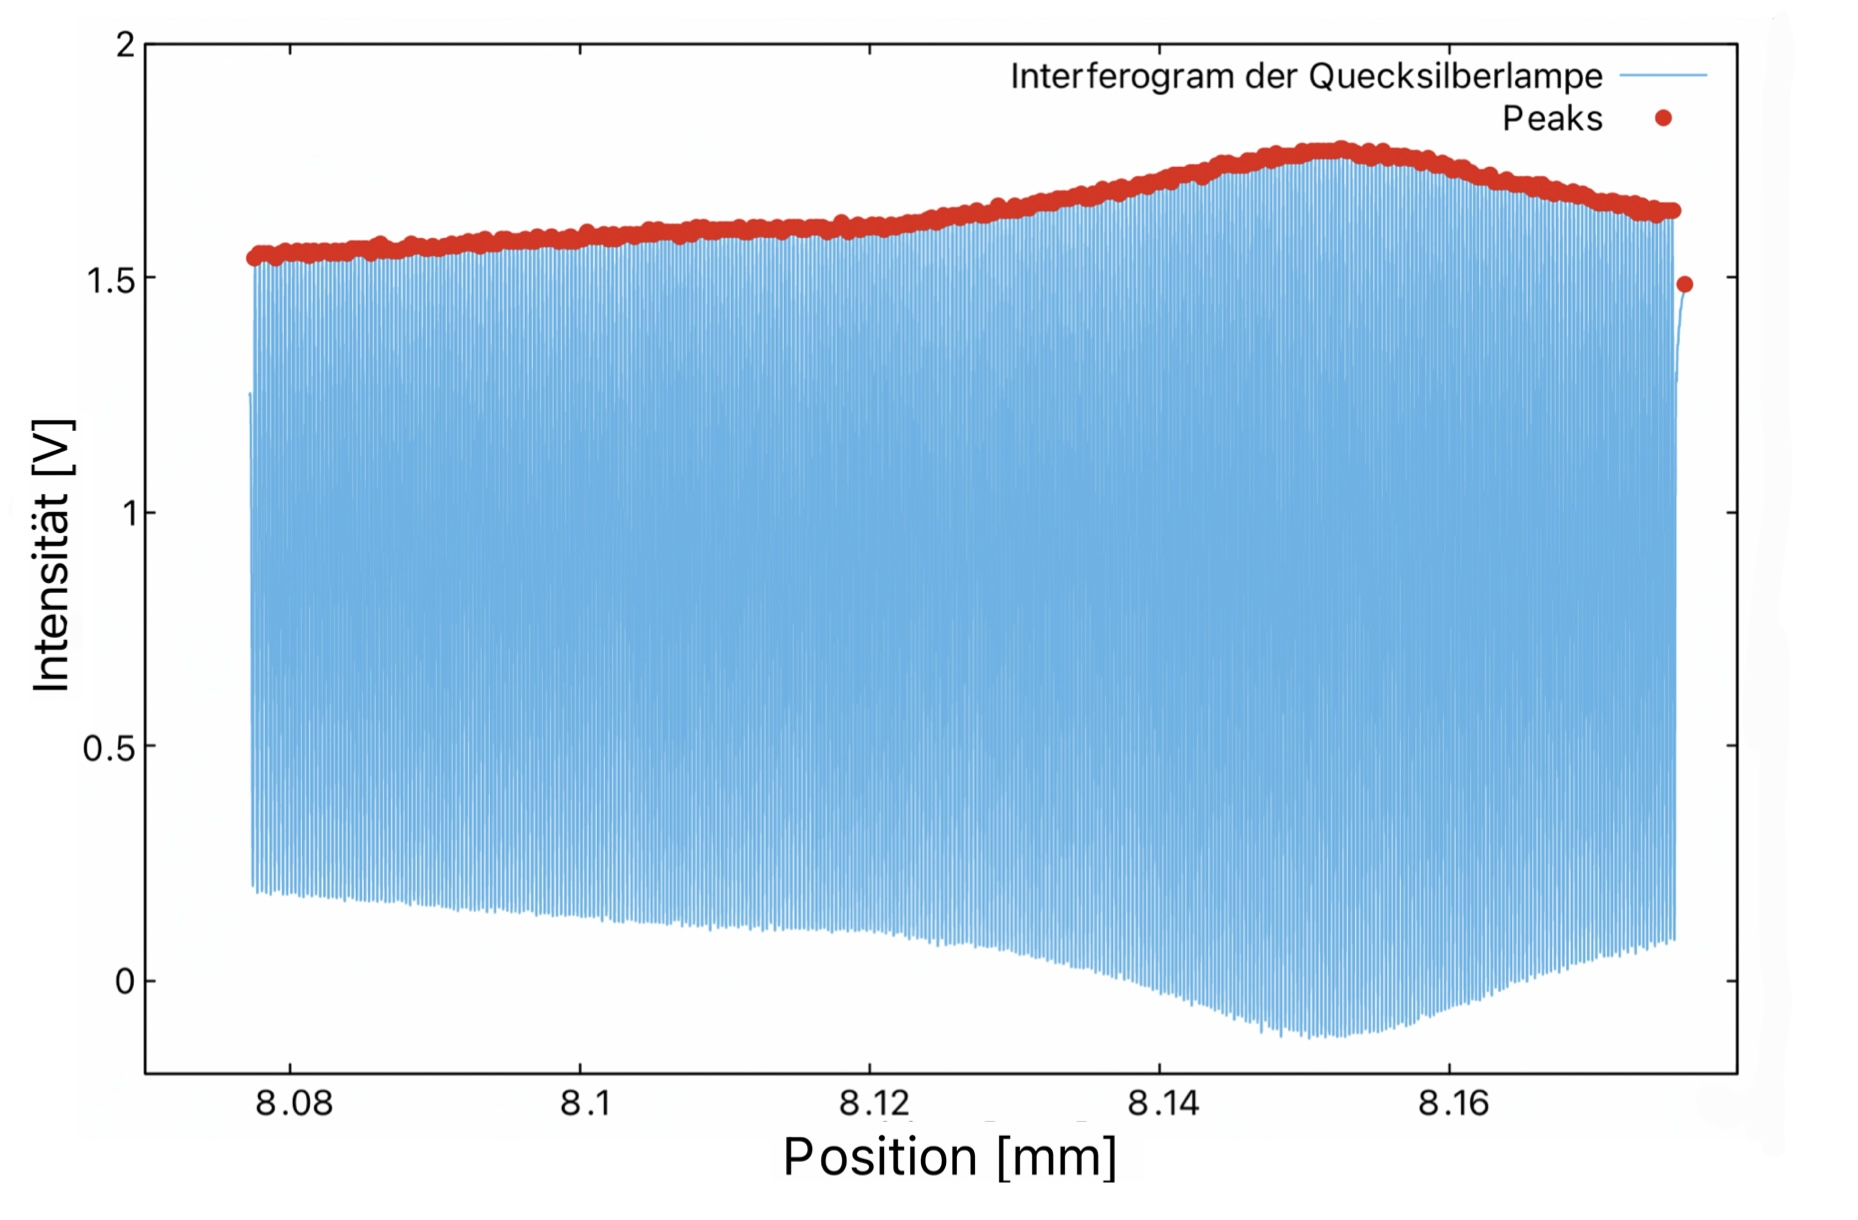
\includegraphics[scale=0.2]{Bilder/Anna/Hg-High-Interferometer.jpg}
    \caption{Interferogramm der Hg-Linie mit den gekennzeichneten Peaks.}
    \label{fig:IHgHigh}
\end{figure}
\begin{figure}[h]
    \centering
    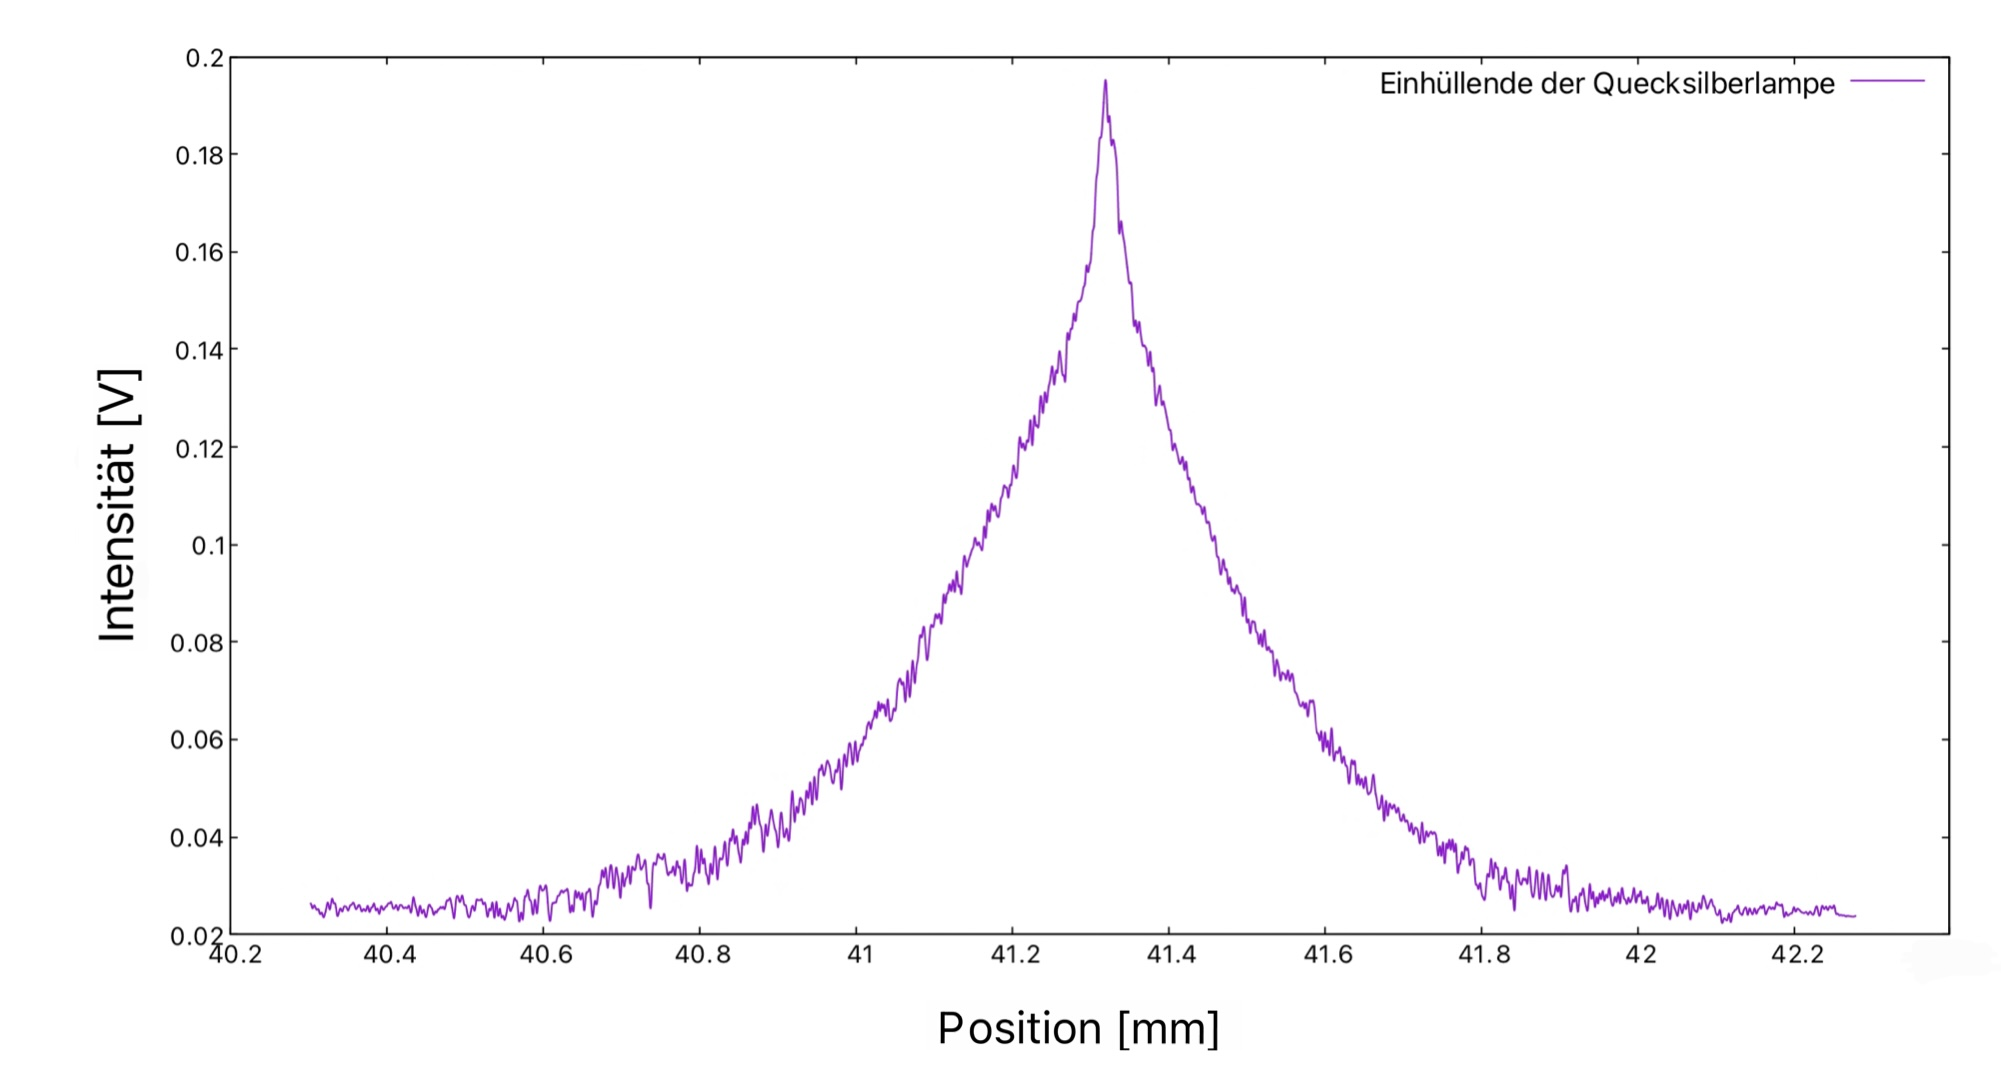
\includegraphics[scale=0.23]{Bilder/Anna/hg-high-ein.jpg}
    \caption{Einhüllende des Interferogramms der Hg-Linie.}
    \label{fig:EHgHigh}
\end{figure}\\
\newpage
\subsection{Wellenlänge}
Die Wellenlänge der Hg-High Lampe wird analog zur Bestimmung der Wellenlänge der Natrium D-Linie bestimmt.\\
Zuerst wurde mithilfe eines Python-Skripts die Peaks des Interferogramms ermittelt, siehe Abbildung \ref{fig:PHgHigh}. 
Die Anzahl der Maxima der Hg-High Lampe beläuft sich auf $n_{Hg-High} = 355$ und die Anzahl der Maxima des Laser 
auf $n_{Laser} = 306$. Die Wellenlänge des Laser ist $\lambda_L = 632,8\,$nm. Somit folgt für die Wellenlänge
der Hg-High Linie:
\begin{equation}
    \lambda_{Hg-High} = \frac{n_{Laser}}{n_{Hg-High}} \lambda_L = 545,4558\,\text{nm}
\end{equation}
Wie bereits bei Natrium Linien besprochen wird auch hier angenommen, dass das Python Skript die Peaks 
bis zu einem Peak genau findet: $s_{n_{Laser}} = s_{n_{Hg-High}} = 1$.\\
Somit folgt für den Fehler:
\begin{align}
    s_{\lambda} &= \sqrt{\left( \frac{\partial \lambda_{Hg-High}}{\partial n_{Laser}}\cdot s_{n_{Laser}}\right)^2+ \left(\frac{\partial \lambda_{Hg-High}}{\partial n_{Hg-High}}\cdot s_{n_{Hg-High}}\right)^2}\\
                &= \sqrt{\left(\frac{\lambda_L}{n_{Hg-High}} \cdot s_{n_{Laser}}\right)^2 + \left(\frac{\lambda_L \cdot n_L}{n^2_{Hg-High}} \cdot s_{n_{Hg-High}}\right)^2 }\\
                &= 2,3533\,\text{nm}
\end{align}
Also ist die Wellenlänge der Quecksilberhochdrucklampe:
\begin{equation}
    \lambda_{Hg-High} = (546 \pm 2)\,\text{nm}
\end{equation}
Der Literaturwert für Quecksilber ist $\lambda_{Hg-Lit} = 546,1\,$nm \citep[vgl.][]{Zusatzliteratur}.\\ Wie man erkennen kann, stimmt
der berechnete Wert und der Literaturwert überein.\\
\begin{figure}[h]
    \centering
    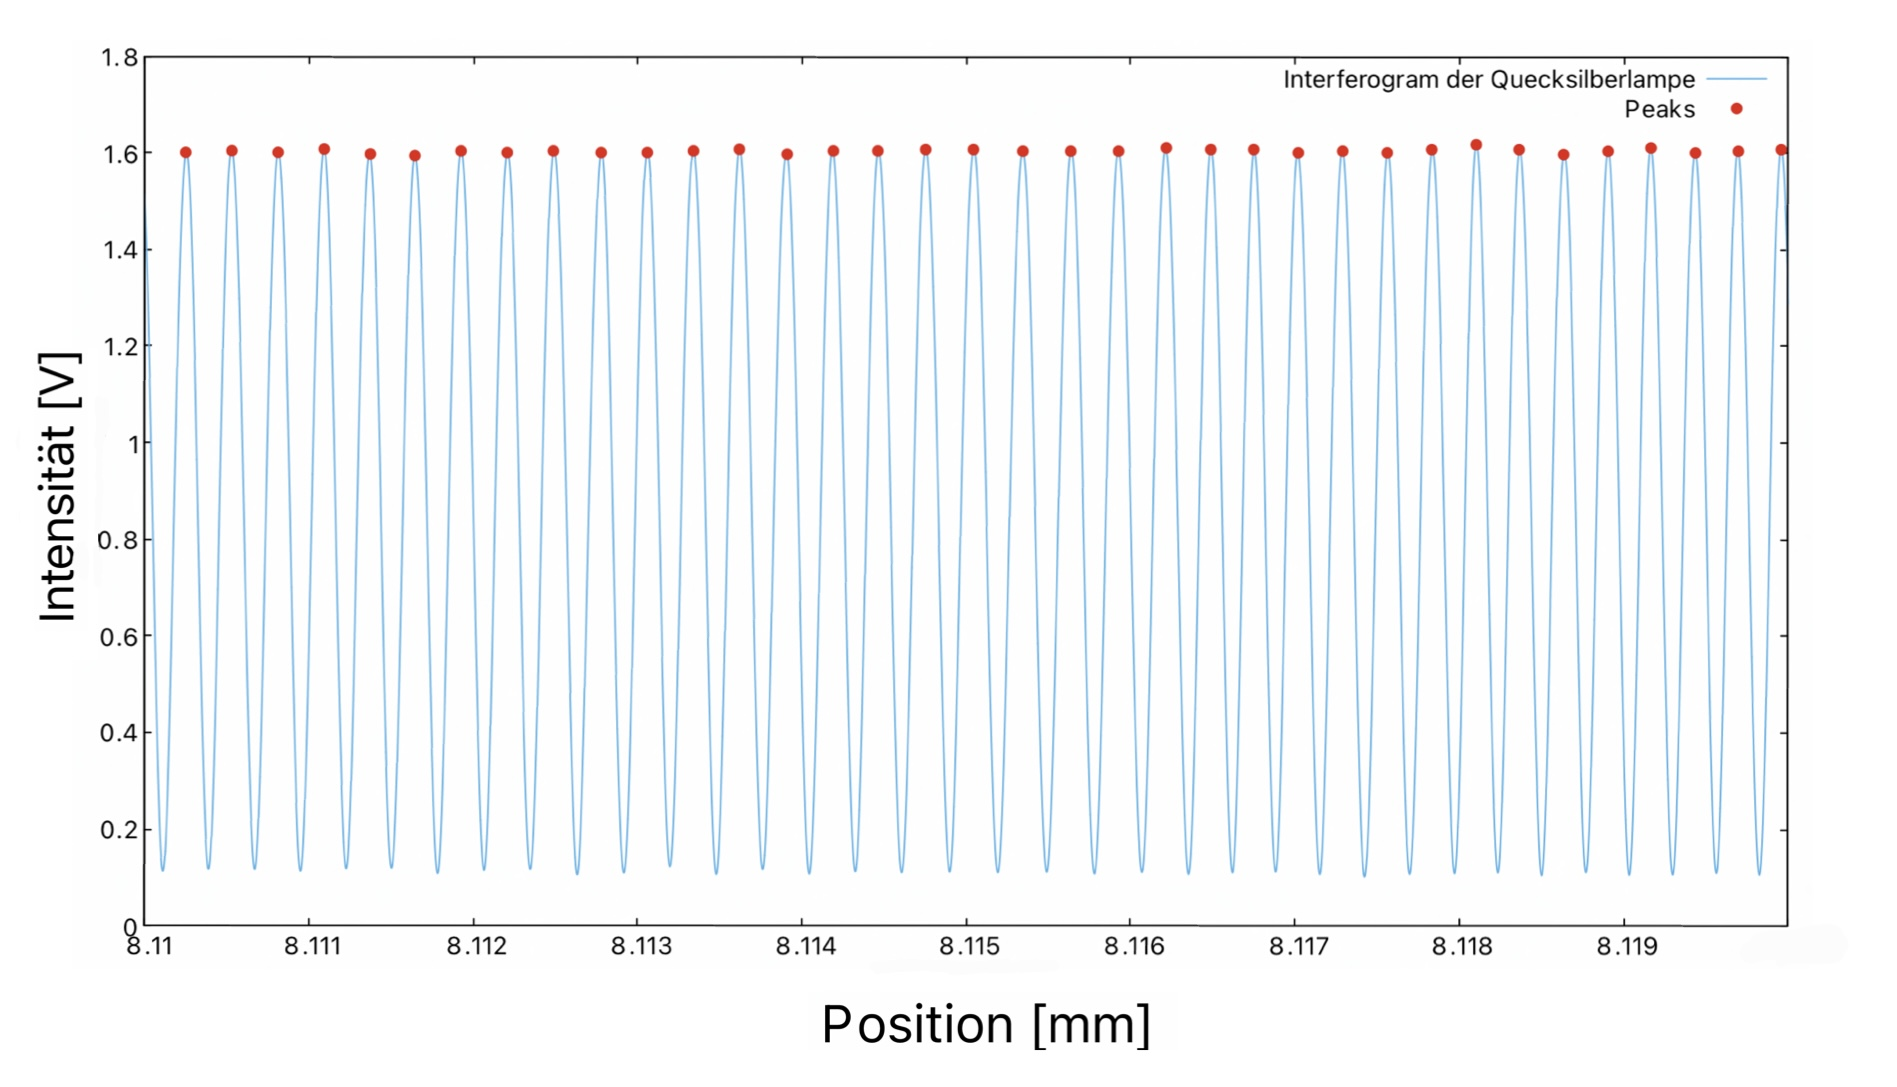
\includegraphics[scale=0.25]{Bilder/Anna/PeaksHigh.jpg}
    \caption{Ausschnitt des Interferogramm der Hg-Linie mit den gekennzeichneten Peaks.}
    \label{fig:PHgHigh}
\end{figure}

\subsection{Kohärenzlänge}
Als nächstes soll die Kohärenzlänge bestimmt werden. Die Kohärenzlänge ist die Länge der halben Halbwertsbreite der Einhüllenden bei der
die maximale Intensität auf $\frac{1}{e}$ abgefallen ist.\\
Die maximale Intensität der Hg-High Lampe beträgt:
\begin{align}
 I_0 = (0,1926 \pm 0,0001)\,\text{V}  \\
 \frac{I_0}{e} = (0,0708 \pm 0,0004)\,\text{V} 
\end{align}
Die maximale Intensität wurde aus dem Plot herausgelesen und anschließend der Offset noch abgezogen, der Ablesefehler wird 
mit $s_{I_0} = 0,0001\,\text{V}$ veranschlagt.\\
Als nächstes muss die Breite der Einhüllenden bestimmt werden bei der die Intensität nur noch $\frac{1}{e}$
beträgt, siehe Abbildung \ref{fig:HgHighf}:
\begin{equation}
    \Delta s_{Hg-High} = 0,4972\,\text{mm}
\end{equation}
Hierbei wird ein Ablesefehler von 0,1 mm angenommen.\\
Nun muss noch der Fehler des Motors 2 berücksichtigt werden, damit man die Kohärenzlänge erhält:
\begin{align}
    L_c = \beta \cdot \frac{\Delta s}{2} = (0,3 \pm 0,1)\,\text{mm}
\end{align}
\begin{figure}[h]
    \centering
    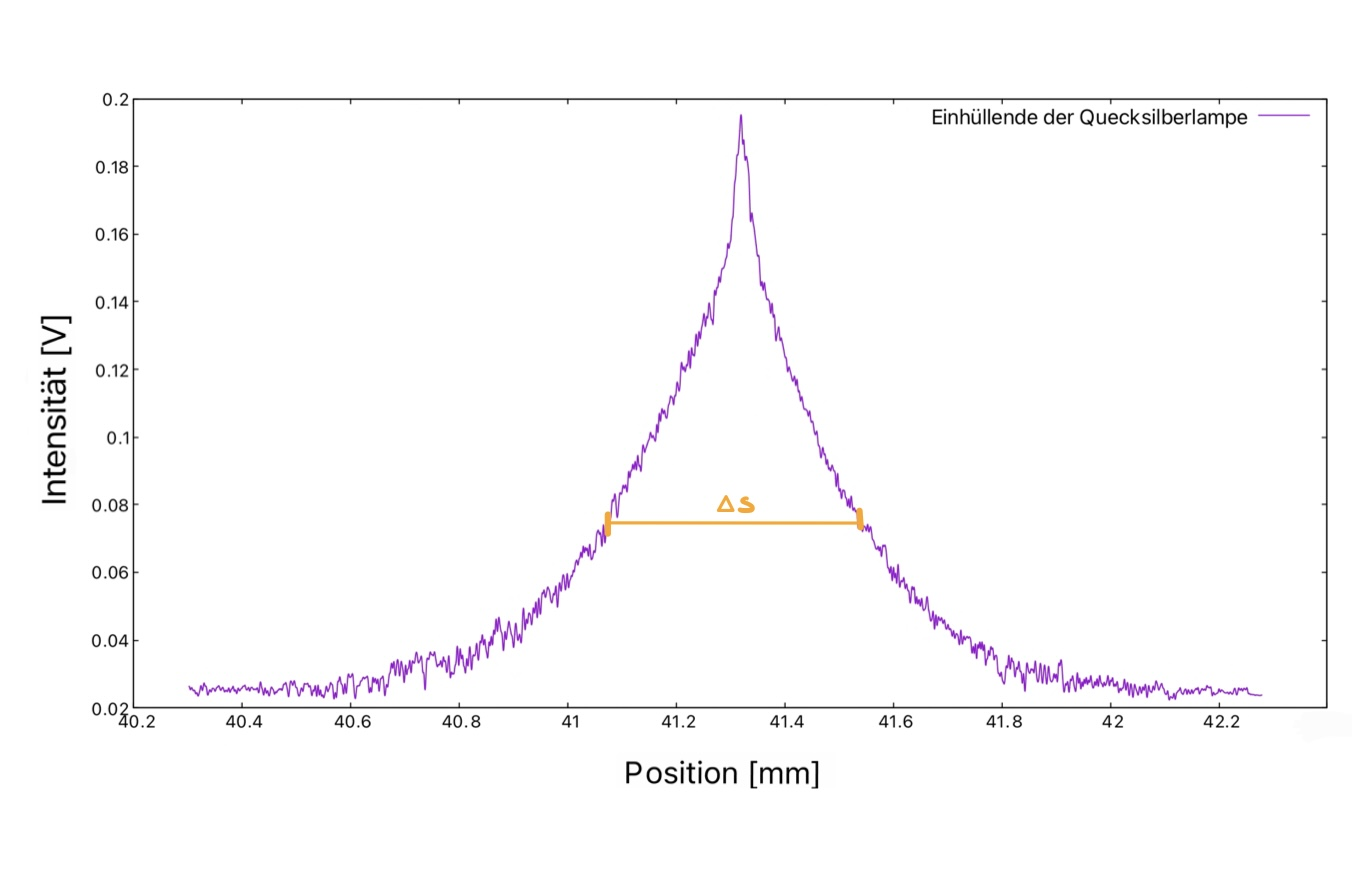
\includegraphics[scale = 0.32]{Bilder/Anna/high1_e.jpg}
    \caption{Einhüllende des Interferogramms der Hg-Linie, zusätzlich wurde noch die Breite, bei der die Intensität nur noch 1/e beträgt, zur Kohärenzlängenbestimmung eingezeichnet.}
    \label{fig:HgHighf}
\end{figure}
\newpage
\subsection{Linienbreite}
Zuletzt soll noch die Linienbreite bestimmt werden.\\
Wie man aus der Abbildung \ref{fig:EHgHigh} erkennen kann, liegt bei der Hg-High Lampe ein Lorentzprofil vor.\\
Somit kann man die Formel für die Halbwertsbreite aus den Fragen zur Vorbereitung (Frage 9) verwenden:
\begin{equation}
    FWHM_{Hg-High} = \frac{2}{L_c} = 8,045 \frac{1}{\text{mm}}
\end{equation}
Die Halbwertsbreite ist in Wellenzahlen angegeben, nun muss sie nur noch in Wellenlänge umgerechnet werden, dies 
geschieht mit der in 3.1.2 hergeleiteten Formel:
\begin{equation}
    \Delta \lambda_{Hg-High} = FWHM \cdot \frac{\lambda^2_{Hg-High}}{2 \cdot \pi} = \frac{2}{L_c} \cdot \frac{\lambda^2_{Hg-High}}{2 \cdot \pi} = \frac{\lambda^2_{Hg-High}}{L_c \cdot \pi} = 0,3810\,\text{nm}
\end{equation}
Der Fehler wird mithilfe der Fehlerfortpflanzung bestimmt:
\begin{align}
    s_{\Delta \lambda_{Hg-High}} &= \sqrt{\left(\frac{\partial \Delta \lambda_{Hg-High}}{\partial L_c} \cdot s_{L_c}\right)^2+\left(\frac{\partial \Delta \lambda_{Hg-High}}{\partial \lambda_{Hg-High}} \cdot s_{\lambda_{Hg-High}}\right)^2} \\
    &= \sqrt{\left(\frac{\lambda^2_{Hg-High}}{L_c^2 \cdot \pi} \cdot s_{L_c}\right)^2+\left(\frac{2\lambda_{Hg-High}}{L_c \cdot \pi} \cdot s_{\lambda_{Hg-High}}\right)^2} \\
    & = 0,01516\,\text{nm}
\end{align}
Hierbei wurden die oben berechneten Fehler für die Kohärenzlänge $s_{L_c}=0,1$\,mm und für die Wellenlänge $s_{\lambda_{Hg-High}}=2,4$\,nm verwendet.\\
Somit ergibt die Halbwertsbreite der Spektrallinie für die Hg-High Lampe:
\begin{equation}
    \Delta \lambda_{Hg-High} = (0,38 \pm 0,02)\,\text{nm}
\end{equation}
Die Einhüllende des Interferogramms der Quecksilberhochdrucklampe ist ein im l-Raum eine abfallende e-Funktion und im k-Raum 
eine Lorentzkurve., siehe auch Abbildung \ref{fig:fithigh}. Das 
heißt allerdings auch, dass diese Linie durch Druck verbreitert wird. In der Abbildung \ref{fig:fithigh} ist 
der l-Raum dargestellt, d.h. eigentlich sollte es eine 1/e Funktion sein, dies ist jedoch wahrscheinlich aufgrund des hohen Alters der Lampe
nicht mehr der Fall.
\begin{figure}[h]
    \centering
    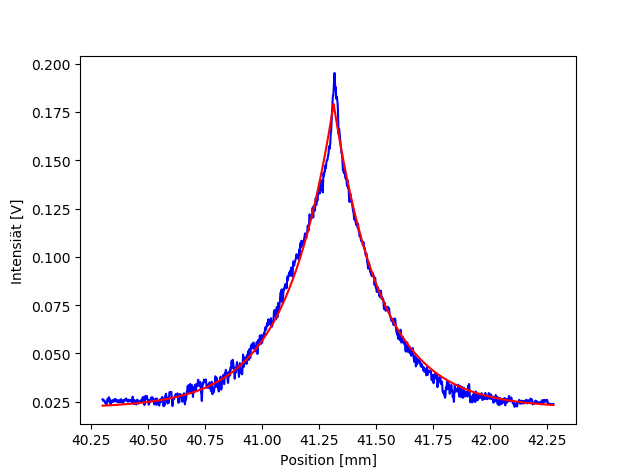
\includegraphics[scale=0.8]{Bilder/Anna/fithigh.png}
    \caption{Einhüllende des Interferogramms der Hg-Linie mit Fit-Funktion.}
    \label{fig:fithigh}
\end{figure}
\newpage